\section{Auswertung}
\label{sec:auswertung}
In diesem Kapitel sollen die aufgenommenen Messwerte ausgewertet werden mit dem Ziel die Suszeptibilität 
zweier Materialien zu bestimmen.
\subsection{Güte des selektiven Verstärkers}
\label{sec:verstaerker}
Um die Güte des selektiven Verstärkers zu bestimmen wurde für unterschiedliche Frequenzen bei gleicher Eingangsspannung 
$U_E$ die verstärkte Spannung gemessen. Das Ergebnis ist im folgenden Diagram \autoref{fig:verstaerker} aufgetragen. 
Um die Güte des Verstärkers zu messen wurde die Kurve auf die Eingangsspannung normiert und die Breite
bei einer Höhe von $\frac{1}{\sqrt{2}}$ bestimmt. Diese liegt bei $\Delta v=\SI[]{695.8}[]{Hz}$. Die Güte lässt sich
mit $v_0=\SI[]{35.5}[]{kHz}$ dann bestimmen über:
\begin{center}
  $Q=\frac{v_0}{\Delta v}=\frac{\SI[]{35.5}[]{kHz}}{\SI[]{0.6958}[]{kHz}}=51.02$
\end{center}
\begin{figure}
    \centering
    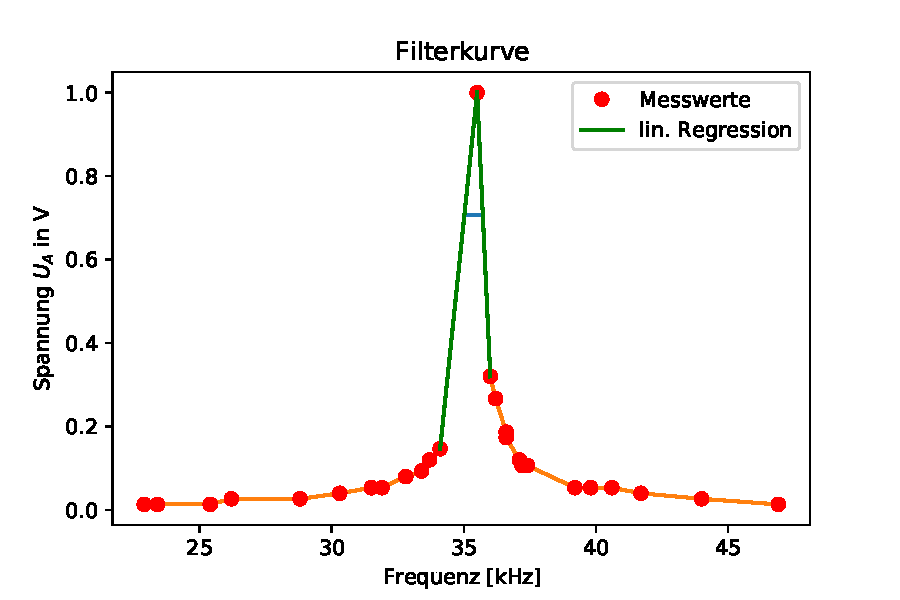
\includegraphics{verstaerker.pdf}
    \caption{Filterkurve des Selektivverstärkers}
    \label{fig:verstaerker}
  \end{figure}
\newpage
\subsection{Berechnung der Suszeptibilität mittels Quantenzahlen}
\label{sec:quantenzahlen}
$Dy^{3+}$ besitzt 9 Elektronen auf der 4f-Schale, es müssen also nach der ersten Hundschen-Regel sieben 
Elektronen einen Spin $\uparrow$ und 2 Elektronen einen Spin $\downarrow$ besitzen es folgt also S=2,5.
Der Gesamtbahndrehimpuls L soll nach der zweiten Hundschen-Regel maximal werden es folgt also L=3+2=5.
Da die Schale nur 14 Elektronen fasst und daher mit neun Elektronen mehr als Halbvoll besetzt ist folgt 
nach der dritten Hundschen-Regel J=L+S=5+2,5=7,5.
Auf gleiche Weise lassen sich für $Gd^{3+}$ die Zahlen S=3,5 , L=0 und J=3,5 herleiten. 
Damit lassen sich über \autoref{eq:landre} die Landé-Faktoren berechnen:
\begin{center}
    $\Rightarrow$ $g_j(Dy^{3+})=1.33$\\
    $g_j(Gd^{3+})=2.00$
\end{center}
Als nächstes werden dann die Momente pro Voulumenanteil $N=\frac{2N_A\rho}{M}$ mit der Dichte $\rho$ und der
molaren Masse M berechnet:

  \begin{table}
    \centering
    
    \caption{Magnetische Momente pro Voulumenanteil}
    \label{tab:moseley}
    \sisetup{table-format=1.2}
    \begin{tabular}{S[table-format=3.2] S S S S  [table-format=3.2]}
      \toprule
      {Material} & {Dichte $\rho$ in $\si[]{\frac{kg}{m^3}}$}&  {M in $\si[]{\frac{kg}{mol}}$}& {N in $\si[]{\frac{1}{m^3}}$}\\
      \midrule
      {$Dy_2 O_3$}& {$7810$} & {$0.373$} & {$2.5218 \times 10^{28}$}\\
      {$Gd_2 O_3$}& {$7410$} & {$0.362$} & {$2.4654 \times 10^{28}$}\\
      \bottomrule
    
    \end{tabular}
  \end{table}

Daraus folgt sofort über \autoref{eq:xi} mit $T=25\si[]{°C}=298.15\si[]{K}$
\begin{center}
    $\mu_B=9.274\times 10^{-24}\si[]{\frac{J}{T}}$\\
    $\mu_0=1.256\times 10^{-6}\si[]{\frac{N}{A^2}}$\\
    $k=1.380\times 10^{-23}\si[]{\frac{J}{K}}$

\end{center}
\begin{center}
    $\chi_{Dy_2 O_3}=24.889\times 10^{-3}$\\
    $\chi_{Gd_2 O_3}=13.593\times 10^{-3}$
\end{center}

\subsection{Berechnung der Suszeptibilität durch Messungen an der Brückenschaltung}
\label{sec:messung}
Zunächst werden die $\Delta R$ berechnet und deren Mittelwert gebildet:
\begin{center}
    $\Delta R_{Dy_2 O_3}=\SI[]{1.55833}[]{\Omega}$\\
    $\Delta R_{Gd_2 O_3}=\SI[]{0.76833}[]{\Omega}$
\end{center}
Als nächstes wird dann $Q_{real}=\frac{m}{l*\rho_w}$ berechnet:
\begin{center}
    $Q_{real, Dy_2 O_3}=1.489 \times 10^{-5}$\\
    $Q_{real, Gd_2 O_3}=1.153 \times 10^{-5}$
\end{center}
Jetzt können mit $\chi=2\frac{\Delta R F}{Q_{real} R_3}$ sofort die Suszeptibilitäten berechnet werden:
\begin{center}
    $\chi_{Dy2 O_3}=18.124 \times 10^{-3}$\\
    $\chi_{Gd2 O_3}=11.540 \times 10^{-3}$
\end{center}


\subsection{Vergleich der Suszeptibilitäten}
\label{sec:vergleich}

\begin{table}
    \centering
    
    \caption{Vergleich der Suszeptibilitäten}
    \label{tab:vergleich}
    \sisetup{table-format=1.2}
    \begin{tabular}{S[table-format=3.2] S S S S  [table-format=3.2]}
      \toprule
      {Material} & { $\chi_{Quantenzahlen}$ in $\si{\frac{m^3}{kg}}$} & {$\chi_{Brückenspannung}$ in $\si{\frac{m^3}{kg}}$} &  {Abweichung in \%}\\
      \midrule
      {$$Dy_2 O_3$$}& {$$24.889\times 10^{-3}$$} & {$$18.124 \times 10^{-3}$$} & {37.3}\\
      {$$Gd_2 O_3$$}& {$$13.593\times 10^{-3}$$} & {$$11.540 \times 10^{-3}$$} & {17.3}\\
      \bottomrule
    
    \end{tabular}
  \end{table}

  Die berechneten Suszeptibilitäten weichen stark von den gemessenen ab.